\begin{problem}[12]
能否用水洞做机翼的模型实验, 或用风洞做潜艇的模型实验? 如果可以, 问尺寸和速度的缩比范围?
\end{problem}
% --------------------------------------------------------------------
\begin{solution}

\noindent\begin{minipage}[c]{0.7\linewidth}
先不具体讨论机翼或潜艇, 统称为固体, 假设固体形状的特征长度是$l, l', \cdots$, 均匀来流速度为$v$, 方位角为$\alpha$, 流体的密度为$\rho$, 粘性系数为$\mu$. 则固体受到流体的作用力$W$可表示为
\end{minipage}
\begin{minipage}[c]{0.3\linewidth}
\begin{center}
%\usetikzlibrary{calc,intersections,through,backgrounds}
\usetikzlibrary{decorations.pathreplacing,decorations.pathmorphing,arrows}
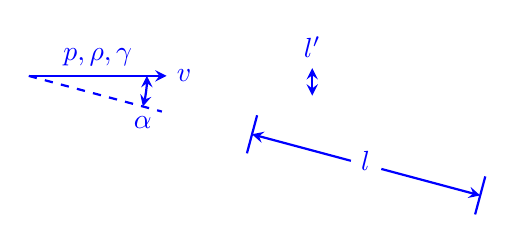
\begin{tikzpicture}
        % Some profiles look better when using plot[smooth]
        \draw[scale=3, rotate=-15, thick]
            plot file{./figures/airfoil.dat} -- cycle;
    \draw[thick,blue] (-0.1,-0.5)--++(-105:0.5) (-0.1,-0.5)++(-15:3)--++(-105:0.5);
	\draw[<-,thick, >=stealth,blue] (-0.1,-0.5)++(-105:0.25) -- ++(-15:1.3) node[right]{$l$};
	\draw[->,thick, >=stealth,blue] (-0.1,-0.5)++(-105:0.25) ++(-15:1.7)--++(-15:1.3);

\draw [->,thick, blue, >=stealth](-3,0)--(-1.25,0) node[right] {$v$} node[above,midway] {$p, \rho, \gamma$}; 
\draw [thick, blue, >=stealth,dashed](-3,0)--++(-15:1.75);
\draw [<->,thick, blue, >=stealth](-1.5,0) arc(0:-15:1.5) node[below] {$\alpha$};
\draw[<->,thick,blue,>=stealth] (0.6,-0.25)--(0.6,0.1) node[above] {$l'$};
\end{tikzpicture}
\usetikzlibrary{%
    decorations.pathreplacing,%
    decorations.pathmorphing,arrows
}

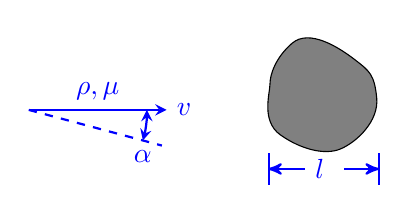
\begin{tikzpicture}


\draw [->,thick, blue, >=stealth](-3,0.85)--(-1.25,0.85) node[right] {$v$} node[above,midway] {$\rho, \mu$}; 
\draw [thick, blue, >=stealth,dashed](-3,0.85)--++(-15:1.75);
\draw [<->,thick, blue, >=stealth](-1.5,0.85) arc(0:-15:1.5) node[below] {$\alpha$};

\begin{scope}[y=0.80pt, x=0.8pt,yscale=-1,yshift=-850]
  \path[draw=black,fill=gray] (12.2092,1002.1870) .. controls (4.7404,1008.6595) and
    (2.2567,1016.3308) .. (2.2567,1020.5208) .. controls (2.2567,1024.7120) and
    (-1.9333,1037.2845) .. (6.9717,1043.5708) .. controls (15.8767,1049.8570) and
    (26.8779,1053.0008) .. (34.2117,1049.8570) .. controls (41.5467,1046.7145) and
    (51.4992,1037.2845) .. (50.4517,1026.8083) .. controls (49.4042,1016.3308) and
    (47.3079,1014.7595) .. (40.4967,1009.5208) .. controls (33.6892,1004.2820) and
    (20.0679,995.3758) .. (12.2092,1002.1870) -- cycle;
\end{scope}

\draw[thick,blue] (0.05,-0.1)--(0.05,0.3) (1.45,-0.1)--(1.45,0.3);
\draw[thick,blue,<-,>=stealth'](0.04,0.1)--(0.51,0.1) node[right] {$l$};
\draw[thick,blue,<-,>=stealth'](1.45,0.1)--(1.0,0.1);
\end{tikzpicture}

\end{center}
\end{minipage}
\[
W = f(l,l',\cdots, v, \alpha; \rho, \mu)
\]
上式中各物理量的量纲分别为:$[l]=[l']=\cdots=L$, $[v]=LT^{-1}$, $\alpha$为无量纲量, $[\rho]=ML^{-3}$, $[\mu]=ML^{-1}T^{-1}$. 选取$l$, $v$, $\rho$作为基本量, 且作为本问题的单位系统, 用以度量问题中的各量. 于是, 得到各量的量值所满足的关系
\[
\frac{W}{\rho v^2 l^2} = f\bigg(1,\frac{l'}{l},\cdots,\alpha,1,\frac{\mu}{\rho vl}\bigg) 
\quad\Longrightarrow\quad
 W = \rho v^2 l^2 f(l'/l,\cdots,\alpha,\mathrm{Re})
\]
如果要用模型实验来求取无量纲函数$f$, 那么在模型(用下标$\mathrm{m}$表示)和原型(用下标$\mathrm{p}$表示)之间, 要满足以下两方面条件
\begin{itemize}
\item 几何相似: $(l'/l,\cdots)_\mathrm{m}=(l'/l,\cdots)_\mathrm{p}$ 及 $\alpha_m = \alpha_p$
\item 动力学相似: $(\mathrm{Re})_\mathrm{m} = (\mathrm{Re})_\mathrm{p}$
\end{itemize}
基于上面对一般情况的分析, 下面分别讨论水洞做机翼的模型实验和风洞做潜艇的模型实验的可行性:
\begin{enumerate}
\item \textbf{水洞做机翼的模型实验:}

世界上最大的水洞一般认为是宾夕法尼亚州立大学的Garfield Thomas水洞\cite{Garfield,wiki_Water_tunnel}, 长$30\mathrm{m}$, 高达$10\mathrm{m}$, 最大水流速度可达$18\mathrm{m/s}$. 而超高速的水洞来流速度可达$84\mathrm{m/s}$\cite{Garfield}. 对于一般的水洞(本题中所考虑的水洞), 直径通常小于$2\mathrm{m}$, 来流速度小于$10\mathrm{m/s}$. 
美国比较流行的CTSW私人小飞机\cite{CTSW}其翼展为$8.5\mathrm{m}$, 全长$6.2\mathrm{m}$, 总高$2.2\mathrm{m}$, 最低巡航速度$65\mathrm{km/h}$. 本题飞机的参数选取主要参考CTSW私人小飞机.
\begin{figure}[!htb]
\centering
\begin{minipage}[t]{.495\linewidth}
\centering
\usetikzlibrary{%
    decorations.pathreplacing,%
    decorations.pathmorphing,arrows
}

\definecolor{ca5bed6}{RGB}{210,210,210}
\definecolor{c1a232b}{RGB}{80,80,80}
\definecolor{c2c3c57}{RGB}{100,100,100}
\definecolor{c354b6b}{RGB}{130,130,130}
\definecolor{c453f41}{RGB}{120,120,120}
\definecolor{caed0e3}{RGB}{250,250,250}
\definecolor{cffffff}{RGB}{255,255,255}


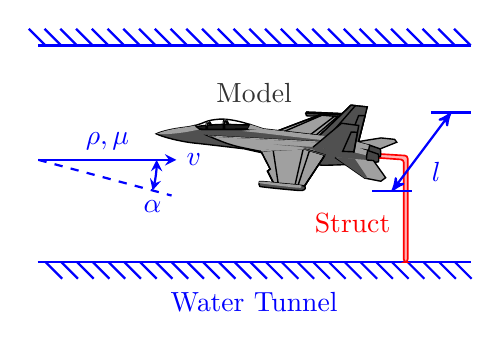
\begin{tikzpicture}[
 interface/.style={
        postaction={draw,decorate,decoration={border,angle=-45,
                    amplitude=0.3cm,segment length=2mm}}}]
\node[blue] at (1.25,-2.5) {Water Tunnel};
\node[black!80] at (1.25,0.15) {Model};
\node[red] at (2.5,-1.5) {Struct};

\draw[thick,interface,blue] (4,0.75)--(-1.5,0.75)  (-1.5,-2)--(4,-2)  ;
\draw[semithick,fill=red!30,draw=red,rounded corners=1](2.8,-0.625)--(3.2,-0.65) --(3.2,-2)--(3.15,-2)--(3.15,-0.7)--(2.8,-0.675)--cycle;
%\draw [->,thick, blue, >=stealth'](-1.5,-0.6)--(-0.35,-0.6) node[above,midway] {$v$} node[below,midway] {$\mu, \rho$};

\begin{scope}[xshift=43,yshift=-20]
\draw [->,thick, blue, >=stealth](-3,0)--(-1.25,0) node[right] {$v$} node[above,midway] {$\rho, \mu$}; 
\draw [thick, blue, >=stealth,dashed](-3,0)--++(-15:1.75);
\draw [<->,thick, blue, >=stealth](-1.5,0) arc(0:-15:1.5) node[below] {$\alpha$};
\end{scope}


\begin{scope}[y=0.80pt, x=0.8pt,yscale=-1,scale=0.2]
\path[draw=black,fill=ca5bed6,line join=miter,line cap=butt,even odd rule,line
  width=0.500pt] (503.2043,101.5802) .. controls (503.9114,101.4035) and
  (544.3933,85.1400) .. (544.3933,85.1400) -- (539.4436,78.5993) --
  (508.8612,75.4173) -- (449.4642,84.9632) -- (474.9201,101.7570) --
  (503.2043,101.5802) -- cycle;
\path[draw=black,fill=c1a232b,line join=miter,line cap=butt,even odd rule,line
  width=0.500pt] (159.1838,44.7695) .. controls (139.1331,44.8015) and
  (109.7113,46.2227) .. (90.2775,50.3633) .. controls (90.4872,50.5531) and
  (90.7081,50.7434) .. (90.9338,50.9258) .. controls (92.3030,52.0322) and
  (93.9063,53.0206) .. (95.6213,53.8320) .. controls (97.3363,54.6434) and
  (99.1788,55.2957) .. (101.0275,55.7383) .. controls (102.8762,56.1809) and
  (104.7260,56.3945) .. (106.4963,56.3945) .. controls (110.0369,56.3945) and
  (134.6684,56.4058) .. (158.7150,56.3320) .. controls (182.7617,56.2583) and
  (206.2223,56.0958) .. (207.4025,55.8008) .. controls (207.9926,55.6533) and
  (208.6762,54.9144) .. (209.3400,53.8633) .. controls (210.0039,52.8122) and
  (210.6562,51.4723) .. (211.2463,50.1445) .. controls (212.1008,48.2218) and
  (212.6378,46.7581) .. (212.9338,45.9258) .. controls (200.0073,45.9013) and
  (184.2746,45.7530) .. (175.8088,45.1758) .. controls (171.9197,44.9106) and
  (166.1167,44.7585) .. (159.1838,44.7695) -- cycle;
\path[draw=black,fill=c2c3c57,line join=miter,line cap=butt,even odd rule,line
  width=0.500pt] (152.7775,51.6758) .. controls (152.1525,39.6758) and
  (153.0073,34.2177) .. (154.9025,33.8008) .. controls (158.0275,33.1133) and
  (160.2775,33.1133) .. (164.7775,44.4883) .. controls (163.6977,45.0120) and
  (163.2148,44.7472) .. (161.6525,44.8633) .. controls (160.4025,40.6133) and
  (158.0275,35.8008) .. (156.9025,36.1758) .. controls (155.7775,36.5508) and
  (155.2775,42.8633) .. (155.5275,47.6758) .. controls (155.6833,50.6743) and
  (155.6525,57.6758) .. (155.6525,57.6758) -- (153.0275,59.6758) --
  (152.7775,51.6758) -- cycle;
\path[draw=black,fill=c2c3c57,line join=miter,line cap=butt,even odd rule,line
  width=0.500pt] (114.0275,56.2383) .. controls (113.4025,44.2383) and
  (114.2775,38.8633) .. (116.1525,38.3633) .. controls (118.0275,37.8633) and
  (121.2775,34.4883) .. (125.7775,45.8633) .. controls (123.8227,45.8245) and
  (123.5273,46.0597) .. (122.2150,46.1133) .. controls (120.9650,41.8633) and
  (119.7536,40.0479) .. (118.6525,40.4883) .. controls (117.0900,41.1133) and
  (116.5275,47.1758) .. (116.7775,51.9883) .. controls (116.9333,54.9868) and
  (116.9025,57.7383) .. (116.9025,57.7383) -- (114.2775,59.7383) --
  (114.0275,56.2383) -- cycle;
\begin{scope}[shift={(-91.47248,-136.26172)}]
  \path[draw=black,fill=c354b6b,line join=miter,line cap=butt,even odd rule,line
    width=0.500pt] (459.6194,162.0047) .. controls (457.8516,162.0047) and
    (433.8100,162.8886) .. (431.8655,161.4744) .. controls (429.9209,160.0602) and
    (430.2745,154.0498) .. (432.2190,153.5195) .. controls (434.1636,152.9891) and
    (529.2694,157.5853) .. (529.2694,157.5853) -- (519.7235,166.0706) --
    (459.6194,162.0047) -- cycle;
  \path[draw=black,fill=ca5bed6,line join=miter,line cap=butt,even odd rule,line
    width=0.500pt] (433.6250,153.4688) .. controls (432.8216,153.4638) and
    (432.3403,153.4981) .. (432.2188,153.5312) .. controls (431.5595,153.7111) and
    (431.0785,154.5156) .. (430.8125,155.5625) .. controls (446.8072,156.8079) and
    (520.5383,160.4307) .. (525.7812,160.6875) -- (529.2812,157.5938) .. controls
    (529.2812,157.5938) and (445.6759,153.5367) .. (433.6250,153.4688) -- cycle;
\end{scope}
\begin{scope}[shift={(-91.47248,-136.26172)}]
  \path[draw=black,fill=ca5bed6,line join=miter,line cap=butt,even odd rule,line
    width=0.500pt] (361.3316,197.7136) -- (461.0336,159.8834) --
    (490.7321,162.3583) -- (509.4704,164.4796) -- (460.6801,211.5022) --
    (361.3316,197.7136) -- cycle;
  \path[draw=black,line join=miter,line cap=butt,line width=0.500pt]
    (495.1250,162.8438) -- (435.8750,208.0625) -- (460.6875,211.5000) --
    (509.4688,164.4688) -- (495.1250,162.8438) -- cycle;
  \path[draw=black,line join=miter,line cap=butt,line width=0.500pt]
    (502.0312,163.6250) -- (448.4062,209.7812) -- (460.6875,211.5000) --
    (509.4688,164.4688) -- (502.0312,163.6250) -- cycle;
  \path[draw=black,line join=miter,line cap=butt,line width=0.500pt]
    (461.0312,159.8750) -- (361.3438,197.7188) -- (375.5000,199.6875) --
    (467.2812,160.4062) -- (461.0312,159.8750) -- cycle;
\end{scope}
\path[draw=black,fill=c354b6b,line join=miter,line cap=butt,even odd rule,line
  width=0.500pt] (87.8088,47.4570) .. controls (81.9341,48.8554) and
  (75.0473,50.2154) .. (65.4963,51.3945) .. controls (17.6980,57.2956) and
  (1.5000,66.1135) .. (1.5000,66.1135) .. controls (12.1287,72.4575) and
  (55.7558,83.8365) .. (87.6213,87.0820) .. controls (119.4868,90.3276) and
  (200.3400,100.0820) .. (200.3400,100.0820) .. controls (200.3400,100.0820) and
  (365.5656,137.2383) .. (376.7775,137.2383) .. controls (387.9895,137.2383) and
  (452.2989,135.1823) .. (465.8713,133.7070) .. controls (479.4436,132.2318) and
  (500.3968,128.8407) .. (500.3968,128.8407) -- (501.2783,112.7557) .. controls
  (501.2783,112.7557) and (498.6405,95.9453) .. (481.5275,91.5195) .. controls
  (464.4146,87.0938) and (454.0900,83.8320) .. (454.0900,83.8320) --
  (382.0900,71.1445) .. controls (382.0900,71.1445) and (248.7207,55.5333) ..
  (244.5900,55.2383) .. controls (242.7873,55.1095) and (229.6445,50.2221) ..
  (213.2150,45.1445) .. controls (213.1364,45.3720) and (212.3706,47.6148) ..
  (211.2463,50.1445) .. controls (210.6562,51.4723) and (210.0039,52.8122) ..
  (209.3400,53.8633) .. controls (208.6762,54.9144) and (207.9926,55.6533) ..
  (207.4025,55.8008) .. controls (206.2223,56.0958) and (182.7617,56.2583) ..
  (158.7150,56.3320) .. controls (134.6684,56.4058) and (110.0369,56.3945) ..
  (106.4963,56.3945) .. controls (104.7260,56.3945) and (102.8762,56.1809) ..
  (101.0275,55.7383) .. controls (99.1788,55.2957) and (97.3363,54.6434) ..
  (95.6213,53.8320) .. controls (93.9063,53.0206) and (92.3030,52.0322) ..
  (90.9338,50.9258) .. controls (89.6381,49.8787) and (88.6100,48.7040) ..
  (87.8088,47.4570) -- cycle;
\path[draw=black,fill=ca5bed6,line join=miter,line cap=butt,even odd rule,line
  width=0.500pt] (117.4235,70.2738) .. controls (146.3384,82.6659) and
  (163.3039,89.7472) .. (188.2356,95.6482) .. controls (213.7928,101.6972) and
  (358.7750,129.2840) .. (358.7750,129.2840) -- (380.0186,108.0403) .. controls
  (380.0186,108.0403) and (387.6900,85.3214) .. (380.3137,84.7313) .. controls
  (372.9374,84.1412) and (118.3086,70.5689) .. (117.4235,70.2738) -- cycle;
\path[fill=c354b6b,even odd rule] (364.5275,96.4883) .. controls
  (355.0275,95.7383) and (266.7775,90.2383) .. (266.7775,90.2383) --
  (326.7775,95.4883) -- (359.0275,102.7383) .. controls (359.0275,102.7383) and
  (360.7775,105.4883) .. (359.2775,104.4883) .. controls (357.7775,103.4883) and
  (332.0275,99.9883) .. (332.0275,99.9883) -- (375.0275,112.4883) --
  (389.0275,127.4883) -- (389.2775,100.4883) -- (364.5275,96.4883) -- cycle;
\path[draw=black,fill=ca5bed6,line join=miter,line cap=butt,even odd rule,line
  width=0.500pt] (258.0900,145.0508) -- (258.4650,145.8008) --
  (252.5588,150.2383) -- (266.1213,177.3633) -- (335.1838,185.3320) --
  (352.0900,159.6758) .. controls (331.0761,156.5846) and (265.2927,146.1906) ..
  (258.0900,145.0508) -- cycle;
\path[draw=black,fill=ca5bed6,line join=miter,line cap=butt,even odd rule,line
  width=0.500pt] (335.1709,185.3436) -- (382.0840,114.2364) .. controls
  (382.0840,114.2364) and (336.6462,100.3690) .. (334.8759,100.0739) .. controls
  (333.1056,99.7789) and (254.0320,103.6145) .. (254.0320,103.6145) --
  (237.8042,105.6799) -- (258.4577,145.8068) -- (252.5567,150.2326) --
  (266.1291,177.3772) -- (335.1709,185.3436) -- cycle;
\path[draw=black,line join=miter,line cap=butt,line width=0.500pt]
  (481.5161,104.7947) -- (446.2575,94.1729);
\path[draw=black,line join=miter,line cap=butt,even odd rule,line width=0.500pt]
  (87.8088,47.4570) .. controls (88.6100,48.7040) and (89.6381,49.8787) ..
  (90.9338,50.9258) .. controls (92.3030,52.0322) and (93.9063,53.0206) ..
  (95.6213,53.8320) .. controls (97.3363,54.6434) and (99.1788,55.2957) ..
  (101.0275,55.7383) .. controls (102.8762,56.1809) and (104.7260,56.3945) ..
  (106.4963,56.3945) .. controls (110.0369,56.3945) and (134.6684,56.4058) ..
  (158.7150,56.3320) .. controls (182.7617,56.2583) and (206.2223,56.0958) ..
  (207.4025,55.8008) .. controls (207.9926,55.6533) and (208.6762,54.9144) ..
  (209.3400,53.8633) .. controls (210.0039,52.8122) and (210.6562,51.4723) ..
  (211.2463,50.1445) .. controls (212.3706,47.6148) and (213.1365,45.3720) ..
  (213.2150,45.1445) .. controls (191.9988,38.5876) and (164.7069,31.5855) ..
  (143.0900,33.0820) .. controls (112.3978,35.2069) and (111.3340,41.8574) ..
  (87.8088,47.4570) -- cycle;
\path[draw=black,line join=miter,line cap=butt,line width=0.500pt]
  (370.2820,69.6837) -- (441.0942,1.5270) -- (477.6805,5.3627) --
  (457.0269,88.5670) -- (367.3315,71.7491) -- (370.2820,69.6837) -- cycle;
\path[draw=black,fill=c354b6b,line join=miter,line cap=butt,even odd rule,line
  width=0.500pt] (370.2820,69.6837) -- (441.0942,1.5270) -- (477.6805,5.3627) --
  (457.0269,88.5670) -- (367.3315,71.7491) -- (370.2820,69.6837) -- cycle;
\path[draw=black,line join=miter,line cap=butt,line width=0.500pt]
  (458.2150,25.1445) -- (435.0900,84.4570) -- (457.0275,88.5820) --
  (472.7775,25.0820) .. controls (471.5501,25.3154) and (458.8960,24.5803) ..
  (458.2150,25.1445) -- cycle;
\path[draw=black,fill=c354b6b,line join=miter,line cap=butt,even odd rule,line
  width=0.500pt] (441.0900,1.5195) -- (370.2775,69.6758) -- (367.3400,71.7383)
  -- (386.6525,75.3633) .. controls (400.1575,60.7299) and (446.9991,7.0632) ..
  (450.9338,2.5508) -- (441.0900,1.5195) -- cycle;
\path[fill=ca5bed6,even odd rule] (213.2150,45.1445) .. controls
  (213.1364,45.3720) and (212.3706,47.6148) .. (211.2463,50.1445) .. controls
  (210.6562,51.4723) and (210.0039,52.8122) .. (209.3400,53.8633) .. controls
  (209.0936,54.2534) and (208.8361,54.5735) .. (208.5900,54.8633) --
  (231.0275,57.3008) .. controls (217.5709,58.3085) and (207.2454,57.6066) ..
  (195.3088,59.6445) .. controls (195.8989,59.9396) and (231.0282,63.1802) ..
  (256.4025,66.4258) .. controls (281.7769,69.6713) and (376.4650,80.3008) ..
  (376.4650,80.3008) -- (415.1520,99.4240) -- (480.9338,116.0195) --
  (490.0588,107.7383) -- (457.0275,97.7070) -- (485.0588,101.8320) --
  (491.4963,96.4570) .. controls (488.8936,94.3730) and (485.6328,92.5812) ..
  (481.5275,91.5195) .. controls (464.4146,87.0938) and (454.0900,83.8320) ..
  (454.0900,83.8320) -- (382.0900,71.1445) .. controls (382.0900,71.1445) and
  (248.7207,55.5333) .. (244.5900,55.2383) .. controls (242.7873,55.1095) and
  (229.6445,50.2221) .. (213.2150,45.1445) -- cycle;
\path[fill=ca5bed6,even odd rule] (122.9154,71.9402) .. controls
  (122.2525,71.7192) and (117.2585,69.7305) .. (117.2585,69.7305) --
  (166.9328,72.5589) -- (371.6402,83.5191) -- (367.6627,86.2591) --
  (122.9154,71.9402) -- cycle;
\path[draw=black,fill=c354b6b,line join=miter,line cap=butt,even odd rule,line
  width=0.500pt] (355.0869,96.3858) -- (419.8505,42.2440) -- (458.5022,47.2599)
  -- (447.4377,108.4829);
\path[draw=black,line join=miter,line cap=butt,line width=0.500pt]
  (441.5275,62.1445) -- (422.2150,105.6758) -- (447.5588,106.8633) --
  (455.6525,62.7383) .. controls (452.0550,62.4619) and (441.5275,62.1445) ..
  (441.5275,62.1445) -- cycle;
\path[draw=black,fill=c453f41,line join=miter,line cap=butt,even odd rule,line
  width=0.500pt] (480.3359,111.2859) .. controls (480.7785,99.7789) and
  (483.2864,91.9600) .. (483.2864,91.9600) .. controls (483.2864,91.9600) and
  (505.8578,99.6314) .. (507.0380,100.2215) .. controls (508.2182,100.8116) and
  (508.5133,117.0394) .. (507.3331,117.4819) .. controls (506.1529,117.9245) and
  (480.9260,120.7275) .. (480.9260,120.7275) -- (480.3359,111.2859) -- cycle;
\path[draw=black,fill=c453f41,line join=miter,line cap=butt,even odd rule,line
  width=0.500pt] (475.9101,123.0879) .. controls (476.3527,111.5809) and
  (478.8606,103.7621) .. (478.8606,103.7621) .. controls (478.8606,103.7621) and
  (501.4320,111.4334) .. (502.6122,112.0235) .. controls (503.7924,112.6136) and
  (504.0875,128.8414) .. (502.9073,129.2840) .. controls (501.7271,129.7265) and
  (476.5002,132.5295) .. (476.5002,132.5295) -- (475.9101,123.0879) -- cycle;
\path[draw=black,fill=ca5bed6,line join=miter,line cap=butt,even odd rule,line
  width=0.500pt] (405.0980,119.5473) .. controls (413.9495,125.7434) and
  (472.0745,166.1653) .. (472.0745,166.1653) -- (508.3657,173.2465) --
  (519.2826,165.2802) -- (491.8429,126.6285) -- (476.2052,125.1532);
\path[draw=black,line join=miter,line cap=butt,line width=0.500pt]
  (333.6838,100.0508) .. controls (333.5469,100.0528) and (333.2795,100.0785) ..
  (333.1213,100.0820) -- (314.3713,182.9257) -- (335.1838,185.3320) --
  (382.0900,114.2382) .. controls (382.0900,114.2382) and (336.6416,100.3770) ..
  (334.8713,100.0820) .. controls (334.7606,100.0636) and (334.3602,100.0389) ..
  (333.6838,100.0508) -- cycle;
\path[draw=black,line join=miter,line cap=butt,line width=0.500pt]
  (347.4338,103.7383) -- (320.9650,183.6758) -- (335.1838,185.3320) --
  (382.0900,114.2383) .. controls (382.0900,114.2383) and (361.4369,107.9344) ..
  (347.4338,103.7383) -- cycle;
\path[draw=black,fill=c354b6b,line join=miter,line cap=butt,even odd rule,line
  width=0.500pt] (271.1449,176.7871) .. controls (271.1449,176.7871) and
  (235.7388,172.6564) .. (234.2636,174.1317) .. controls (232.7883,175.6069) and
  (232.4933,183.8684) .. (235.1487,185.0486) .. controls (237.8042,186.2288) and
  (328.0897,195.3753) .. (330.4501,194.1951) .. controls (337.4820,193.3171) and
  (341.6620,186.4550) .. (333.9907,183.5733) .. controls (327.4996,181.5079) and
  (270.8499,177.3772) .. (271.1449,176.7871) -- cycle;
\path[draw=black,line join=miter,line cap=butt,line width=0.500pt]
  (265.1838,103.0820) .. controls (262.5015,103.2111) and (254.0275,103.6133) ..
  (254.0275,103.6133) -- (237.8088,105.6758) -- (258.4650,145.8008) --
  (252.5588,150.2383) -- (266.1213,177.3633) -- (276.6838,178.5820) --
  (265.1838,103.0820) -- cycle;
\path[fill=ca5bed6,even odd rule] (87.7775,47.4570) .. controls
  (81.9090,48.8530) and (75.0319,50.2173) .. (65.4963,51.3945) .. controls
  (26.2169,56.2438) and (8.0757,63.5873) .. (2.7775,66.0820) .. controls
  (19.8454,69.0879) and (56.0765,63.8694) .. (64.3713,62.7383) .. controls
  (73.5511,61.4865) and (97.6765,56.3728) .. (97.6765,56.3728) .. controls
  (97.6765,56.3728) and (88.6506,51.1753) .. (88.9963,49.3945) .. controls
  (89.0678,49.0259) and (88.3018,48.3435) .. (87.7775,47.4570) -- cycle;
\path[fill=c354b6b,even odd rule] (405.3027,119.0615) -- (412.9025,124.5508) ..
  controls (429.4047,136.0551) and (472.0900,166.1758) .. (472.0900,166.1758) --
  (476.1525,166.9570) -- (476.3400,162.2070) -- (449.5275,122.5508) --
  (405.3027,119.0615) -- cycle;
\path[fill=ca5bed6,even odd rule] (236.4483,102.2873) .. controls
  (239.6303,107.5906) and (240.5142,106.5300) .. (240.5142,106.5300) .. controls
  (240.5142,106.5300) and (264.2022,103.7015) .. (268.0913,104.0551) .. controls
  (271.9804,104.4086) and (335.4432,101.4035) .. (335.4432,101.4035) --
  (344.1053,101.2267) .. controls (344.1053,101.2267) and (324.8366,96.8073) ..
  (323.7760,96.4537) .. controls (322.7153,96.1002) and (236.6251,102.2873) ..
  (236.4483,102.2873) -- cycle;
\path[fill=c354b6b,even odd rule] (385.6478,115.8991) .. controls
  (364.0811,110.5958) and (336.1504,101.4035) .. (336.1504,101.4035) --
  (341.1001,101.2267) -- (386.8853,114.4849) -- (386.5317,116.9598) --
  (385.6478,115.8991) -- cycle;
\path[fill=ca5bed6,even odd rule] (236.2775,173.8320) .. controls
  (235.1682,173.8602) and (234.4619,173.9601) .. (234.2775,174.1445) .. controls
  (233.8416,174.5805) and (233.5242,175.6313) .. (233.3400,176.8945) --
  (234.7775,177.7383) .. controls (304.0275,186.7383) and (325.0275,188.7383) ..
  (328.0275,187.7383) .. controls (329.7513,187.1637) and (329.7226,184.7071) ..
  (329.4025,182.7070) .. controls (314.2149,180.5247) and (270.8944,177.3171) ..
  (271.1525,176.8008) .. controls (271.1525,176.8008) and (244.0428,173.6344) ..
  (236.2775,173.8320) -- cycle;
\path[fill=caed0e3,even odd rule] (116.7150,39.6758) .. controls
  (118.4931,38.2989) and (119.5377,38.6884) .. (121.8400,39.6133) .. controls
  (121.8400,39.6133) and (119.8766,38.0508) .. (119.3766,38.0508) .. controls
  (114.4090,38.3171) and (114.6992,40.7502) .. (114.4650,47.1133) .. controls
  (114.9302,46.8733) and (114.1137,47.4614) .. (115.3950,47.0626) .. controls
  (115.0412,43.4376) and (116.1666,40.7702) .. (116.7150,39.6758) -- cycle;
\path[fill=caed0e3,even odd rule] (160.4025,36.3008) .. controls
  (160.4025,36.3008) and (158.0275,34.1133) .. (157.5275,34.1133) .. controls
  (157.0275,34.1133) and (155.0275,34.1133) .. (154.6525,34.4883) .. controls
  (152.7287,37.6047) and (153.3015,39.8640) .. (153.1525,42.6758) .. controls
  (153.8670,42.5710) and (152.8332,42.5386) .. (153.8005,42.6571) .. controls
  (153.4736,31.2785) and (157.9575,34.5760) .. (160.4025,36.3008) -- cycle;
\end{scope}

\draw[thick,blue] (2.75,-1.1)--(3.25,-1.1)  (3.5,-0.1)--(4,-0.1);
\draw[thick,blue,<->,>=stealth'](3,-1.1)--(3.75,-0.1) node[midway,below right]{$l$};

\end{tikzpicture}
 
\caption{\label{fig:3dAircraftModeling}三维飞机的水洞模拟}
\end{minipage}
\begin{minipage}[t]{.495\linewidth}
\centering
\usetikzlibrary{calc,intersections,through,backgrounds}
\usetikzlibrary{decorations.pathreplacing,decorations.pathmorphing,arrows}
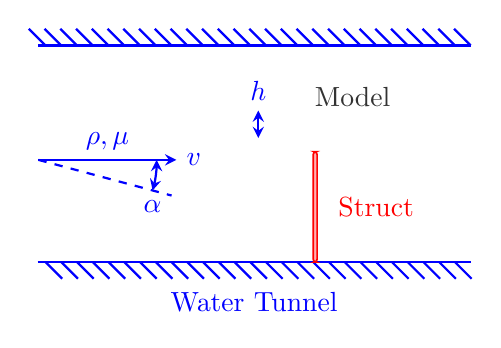
\begin{tikzpicture}[
 interface/.style={
        postaction={draw,decorate,decoration={border,angle=-45,
                    amplitude=0.3cm,segment length=2mm}}}]
\node[blue] at (1.25,-2.5) {Water Tunnel};
\node[black!80] at (2.5,0.1) {Model};
\node[red] at (2.8,-1.3) {Struct};

\draw[thick,interface,blue] (4,0.75)--(-1.5,0.75)  (-1.5,-2)--(4,-2)  ;
\draw[semithick,fill=red!30,draw=red,rounded corners=1](2,-0.6) --(2,-2)--(2.05,-2)--(2.05,-0.6)--cycle;

\begin{scope}[xshift=20,yshift=-5]
% Some profiles look better when using plot[smooth]
 \draw[scale=3, rotate=-15, thick]
            plot file{./figures/airfoil.dat} -- cycle;
\draw[<->,thick,blue,>=stealth] (0.6,-0.25)--(0.6,0.1) node[above] {$h$};
\end{scope}
\begin{scope}[xshift=43,yshift=-20]
\draw [->,thick, blue, >=stealth](-3,0)--(-1.25,0) node[right] {$v$} node[above,midway] {$\rho, \mu$}; 
\draw [thick, blue, >=stealth,dashed](-3,0)--++(-15:1.75);
\draw [<->,thick, blue, >=stealth](-1.5,0) arc(0:-15:1.5) node[below] {$\alpha$};
\end{scope}


\end{tikzpicture}
\caption{\label{fig:2dAircraftModeling}二维翼形的水洞模拟}
\end{minipage}
\end{figure}

表\ref{tab:airfoilINwater}列出了低速小飞机在空气中飞行的参数范围和水洞实验允许的参数值, 以及空气和水的运动粘性系数\cite{fluid_Properties}. 做机翼的模型实验, 考虑到实验时模型的放置方式, 三维模拟时, 尺寸应以翼展方向的缩比为准; 二维模拟时, 尺寸应以翼型厚度方向的缩比为准. \textcolor{blue}{为消除边界影响, 模型的厚度不应大于水洞直径的1/5}.

\begin{table}[!htb]\label{tab:airfoilINwater}
\centering
\caption{水洞做机翼的模型实验与原型的各参量范围}
\begin{tabular}{l|c|c}
\hline 
 & 原型参数实际范围 & 模型参数允许范围\tabularnewline
\hline 
翼展长度$l\,(\mathrm{m})$ & $>8.0$ & $<2.0$\tabularnewline
翼形厚度$h\,(\mathrm{m})$ & $>0.2$ & \textcolor{blue}{$<2/5$}\tabularnewline
\hline 
$v\,(\mathrm{m/s})$ & $>20$ & $<10$\tabularnewline
\hline 
$\nu=\mu/\rho\,(\mathrm{m^{2}/s})$ & $1.5\times 10^{-5}$ & $1.0\times 10^{-6}$\tabularnewline
\hline 
$\mathrm{Re_{3d}} = vl/\nu$ & $>1.0\times 10^7$ & $<2.0\times 10^7$\tabularnewline
$\mathrm{Re_{2d}} = vh/\nu$ & $>1.3\times 10^5$ & $<4\times 10^6$ \tabularnewline
\hline 
\end{tabular}
\end{table}

用表\ref{tab:airfoilINwater}中的参数可分别计算出原型和模型中的几何相似和动力学无量纲相似参数, 几何相似容易满足, 主要考查动力学相似, 通过计算原型和模型中雷诺数的范围(三维和二维模拟情况下的雷诺数范围见表\ref{tab:airfoilINwater}最后两列). \textbf{三维模拟}情况下, 尺寸缩比和速度缩比范围满足以下条件
\[
\alpha_l = \frac{l_\mathrm{p}}{l_\mathrm{m}} > \frac{8}{2}\, , 
\quad 
\alpha_v = \frac{v_\mathrm{p}}{v_\mathrm{m}} > \frac{20}{10}\, , 
\quad 
\alpha_l\cdot \alpha_v = \frac{\nu_\mathrm{p}}{\nu_\mathrm{m}}  = 15
\]
由此可解得尺寸缩比和速度缩比范围分别为
\[
\alpha_l \in (4, 15/2), \qquad \alpha_v \in (2, 15/4)
\]
因此在做三维模拟时, 水洞可以用来模拟翼展长度$l<15\mathrm{m}$, 速度$v<37.5\mathrm{m/s}$的飞机. 若把机翼简化成二维模型, 则可以模拟尺寸更大, 速度更快的飞机. 二维情况下, 尺寸缩比和速度缩比范围满足以下条件
\[
\alpha_l = \frac{h_\mathrm{p}}{h_\mathrm{m}} > \frac{0.2}{2/5}\, , 
\quad 
\alpha_v = \frac{v_\mathrm{p}}{v_\mathrm{m}} >\frac{20}{10}\, , 
\quad 
\alpha_l\cdot \alpha_v = \frac{\nu_\mathrm{p}}{\nu_\mathrm{m}}  = 15
\]
由此可解得尺寸缩比和速度缩比范围分别为
\[
\alpha_l \in (1/2, 15/2), \qquad \alpha_v \in (2, 30)
\]
因此在做\textbf{二维模拟}时, 水洞可以用来模拟翼形高度$h<3\mathrm{m}$, 速度$v<300\mathrm{m/s}$的飞机. 二维模拟能模拟飞机的尺寸和速度比三维模拟的范围更大.

\item \textbf{风洞做潜艇的模型实验:}

\begin{minipage}[c]{0.6\linewidth}

%世界上最大的潜艇是Typhoons\cite{Typhoon}, 长$175\mathrm{m}$, 宽$23\mathrm{m}$, 速度可达$41.15\mathrm{km/h}$.
芬兰海军的Saukko\cite{Saukko}潜艇是世界上最小的潜艇之一, 其长为$32.4\mathrm{m}$, 宽为$4.1\mathrm{m}$, 速度为$10.6\mathrm{km/h}$. 世界上最快的潜艇一般认为是苏联K-222潜艇\cite{K-222}, 速度可达$82.8\mathrm{km/h}$. 低速风洞的直径一般小于$6\mathrm{m}$\cite{baike_wind_tunnel,wike_wind_tunnel}, \textcolor{blue}{为消除边界影响, 模型的宽度不应大于风洞直径的1/3}, \textcolor{red}{这里限制风洞马赫数低于0.3, 即风洞的气流速度低于$100\mathrm{m/s}$}. 
\end{minipage}
\begin{minipage}[c]{0.4\linewidth}
\begin{center}
\usetikzlibrary{%
    decorations.pathreplacing,%
    decorations.pathmorphing,arrows
}

\definecolor{ca5bed6}{RGB}{160,160,160}
\definecolor{c1a232b}{RGB}{30,30,30}
\definecolor{c2c3c57}{RGB}{50,50,50}
\definecolor{c354b6b}{RGB}{80,80,80}
\definecolor{c453f41}{RGB}{70,70,70}
\definecolor{caed0e3}{RGB}{200,200,200}
\definecolor{cffffff}{RGB}{255,255,255}


\definecolor{ceb2f9e}{RGB}{150,150,150}
\definecolor{c231f20}{RGB}{30,30,30}
\definecolor{cf188c6}{RGB}{180,180,180}
\definecolor{cfac2e3}{RGB}{220,220,220}
\definecolor{cec008c}{RGB}{60,60,60}
\definecolor{cf9b2dc}{RGB}{200,200,200}


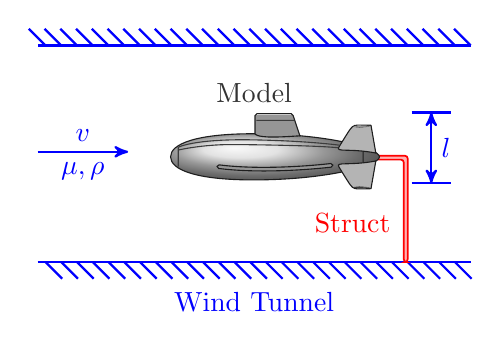
\begin{tikzpicture}[
 interface/.style={
        postaction={draw,decorate,decoration={border,angle=-45,
                    amplitude=0.3cm,segment length=2mm}}}]
\node[blue] at (1.25,-2.5) {Wind Tunnel};
\node[black!80] at (1.25,0.15) {Model};
\node[red] at (2.5,-1.5) {Struct};

\draw[thick,interface,blue] (4,0.75)--(-1.5,0.75)  (-1.5,-2)--(4,-2)  ;
\draw[semithick,fill=red!30,draw=red,rounded corners=1](2.8,-0.65)--(3.2,-0.65) --(3.2,-2)--(3.15,-2)--(3.15,-0.7)--(2.8,-0.7)--cycle;
\draw [->,thick, blue, >=stealth'](-1.5,-0.6)--(-0.35,-0.6) node[above,midway] {$v$} node[below,midway] {$\mu, \rho$};

\draw[thick,blue](3.25,-0.1)--(3.75,-0.1) (3.25,-1)--(3.75,-1);
\draw[thick,blue,<->,>=stealth'] (3.5,-0.1)--(3.5,-1) node[midway,right] {$l$};

\begin{scope}[y=0.80pt, x=0.8pt,yscale=-1,yshift=-1231,xshift=4,scale=1.5]
  \begin{scope}[cm={{0.125,0.0,0.0,-0.125,(-449.47783,1529.2107)}}]
      \path[ball color = gray!30] (4108.1200,3901.0700) .. controls
        (4108.1200,3880.5400) and (3981.6500,3845.4700) .. (3803.9100,3845.4700) ..
        controls (3664.9500,3845.4700) and (3604.9100,3870.3700) ..
        (3604.9100,3901.0700) .. controls (3604.9100,3931.8000) and
        (3664.9500,3956.7000) .. (3803.9100,3956.7000) .. controls
        (3981.6500,3956.7000) and (4108.1200,3921.9500) .. (4108.1200,3901.0700);
      \path[nonzero rule] (4108.1200,3901.0700) .. controls (4108.1200,3880.5400) and
        (3981.6500,3845.4700) .. (3803.9100,3845.4700) .. controls
        (3664.9500,3845.4700) and (3604.9100,3870.3700) .. (3604.9100,3901.0700) ..
        controls (3604.9100,3931.8000) and (3664.9500,3956.7000) ..
        (3803.9100,3956.7000) .. controls (3981.6500,3956.7000) and
        (4108.1200,3921.9500) .. (4108.1200,3901.0700);
  \end{scope}
  \begin{scope}[cm={{0.125,0.0,0.0,-0.125,(-449.47783,1529.2107)}}]
      \path[draw=c231f20] (4108.1200,3901.0700) .. controls (4108.1200,3880.5400) and
        (3981.6500,3845.4700) .. (3803.9100,3845.4700) .. controls
        (3664.9500,3845.4700) and (3604.9100,3870.3700) .. (3604.9100,3901.0700) ..
        controls (3604.9100,3931.8000) and (3664.9500,3956.7000) ..
        (3803.9100,3956.7000) .. controls (3981.6500,3956.7000) and
        (4108.1200,3921.9500) .. (4108.1200,3901.0700) -- cycle;
  \end{scope}
  \begin{scope}[cm={{0.125,0.0,0.0,-0.125,(-449.47783,1529.2107)}}]
      \path[fill=ceb2f9e] (3916.4700,3951.7500) .. controls
        (3916.4700,3951.7500) and (3875.5400,3948.7200) .. (3851.8000,3948.7200) ..
        controls (3808.8500,3948.7200) and (3808.3500,3956.6100) ..
        (3808.3500,3956.6100) -- (3808.3500,4000.4500) .. controls
        (3808.3500,4002.8400) and (3810.3000,4004.8000) .. (3812.7000,4004.8000) --
        (3895.9600,4004.8000) .. controls (3898.3400,4004.8000) and
        (3900.3100,4002.8400) .. (3900.3100,4000.4500) -- (3916.4700,3951.7500);
      \path (3916.4700,3951.7500) .. controls (3916.4700,3951.7500) and
        (3875.5400,3948.7200) .. (3851.8000,3948.7200) .. controls
        (3808.8500,3948.7200) and (3808.3500,3956.6100) .. (3808.3500,3956.6100) --
        (3808.3500,4000.4500) .. controls (3808.3500,4002.8400) and
        (3810.3000,4004.8000) .. (3812.7000,4004.8000) -- (3895.9600,4004.8000) ..
        controls (3898.3400,4004.8000) and (3900.3100,4002.8400) ..
        (3900.3100,4000.4500) -- (3916.4700,3951.7500);
  \end{scope}
  \begin{scope}[cm={{0.125,0.0,0.0,-0.125,(-449.47783,1529.2107)}}]
      \path[draw=c231f20] (3916.4700,3951.7500) .. controls (3916.4700,3951.7500) and
        (3875.5400,3948.7200) .. (3851.8000,3948.7200) .. controls
        (3808.8500,3948.7200) and (3808.3500,3956.6100) .. (3808.3500,3956.6100) --
        (3808.3500,4000.4500) .. controls (3808.3500,4002.8400) and
        (3810.3000,4004.8000) .. (3812.7000,4004.8000) -- (3895.9600,4004.8000) ..
        controls (3898.3400,4004.8000) and (3900.3100,4002.8400) ..
        (3900.3100,4000.4500) -- (3916.4700,3951.7500) -- cycle;
  \end{scope}
  \begin{scope}[cm={{0.125,0.0,0.0,-0.125,(-449.47783,1529.2107)}}]
      \path[fill=cf188c6] (4099.3700,3910.3200) -- (4087.7400,3977.0100)
        .. controls (4087.7400,3977.0100) and (4073.1100,3977.5100) ..
        (4061.9900,3977.5100) .. controls (4050.8700,3977.5100) and
        (4045.3100,3978.0300) .. (4038.2400,3968.4200) .. controls
        (4031.1700,3958.8300) and (4012.8100,3928.3100) .. (4010.4500,3924.4700) ..
        controls (4002.3600,3911.3300) and (4034.7000,3922.4400) ..
        (4099.3700,3910.3200);
      \path(4099.3700,3910.3200) -- (4087.7400,3977.0100) .. controls
        (4087.7400,3977.0100) and (4073.1100,3977.5100) .. (4061.9900,3977.5100) ..
        controls (4050.8700,3977.5100) and (4045.3100,3978.0300) ..
        (4038.2400,3968.4200) .. controls (4031.1700,3958.8300) and
        (4012.8100,3928.3100) .. (4010.4500,3924.4700) .. controls
        (4002.3600,3911.3300) and (4034.7000,3922.4400) .. (4099.3700,3910.3200);
  \end{scope}
  \begin{scope}[cm={{0.125,0.0,0.0,-0.125,(-449.47783,1529.2107)}}]
      \path[draw=c231f20] (4099.3700,3910.3200) -- (4087.7400,3977.0100) .. controls
        (4087.7400,3977.0100) and (4073.1100,3977.5100) .. (4061.9900,3977.5100) ..
        controls (4050.8700,3977.5100) and (4045.3100,3978.0300) ..
        (4038.2400,3968.4200) .. controls (4031.1700,3958.8300) and
        (4012.8100,3928.3100) .. (4010.4500,3924.4700) .. controls
        (4002.3600,3911.3300) and (4034.7000,3922.4400) .. (4099.3700,3910.3200) --
        cycle;
      \path[fill=cfac2e3] (4086.3200,3975.5000) .. controls
        (4086.3200,3975.5000) and (4061.5900,3976.0400) .. (4056.6900,3976.0400) ..
        controls (4051.8000,3976.0400) and (4047.7200,3975.2300) ..
        (4045.5500,3973.6000) .. controls (4045.5500,3973.6000) and
        (4051.8000,3973.0600) .. (4063.2100,3973.3300) .. controls
        (4074.6300,3973.6000) and (4086.3200,3975.5000) .. (4086.3200,3975.5000);
      \path[fill=cec008c] (4085.5100,3975.2300) .. controls
        (4082.0800,3973.9400) and (4078.1800,3974.3200) .. (4074.6300,3973.6300) ..
        controls (4072.1000,3973.1400) and (4069.6300,3972.8400) ..
        (4067.0200,3972.7900) .. controls (4064.3200,3972.7400) and
        (4061.5400,3972.6300) .. (4058.8500,3972.7900) .. controls
        (4056.6600,3972.9200) and (4053.2500,3972.6000) .. (4051.3500,3973.6200) ..
        controls (4058.4300,3973.7100) and (4065.5400,3973.2900) ..
        (4072.5700,3974.0100) .. controls (4074.9800,3974.2500) and
        (4077.4700,3974.2400) .. (4079.8100,3974.6800) .. controls
        (4081.6600,3975.0400) and (4084.3400,3974.8300) .. (4086.0500,3975.5000);
      \path[fill=cec008c] (4053.9800,3972.7800) .. controls
        (4051.5200,3971.5000) and (4047.5100,3973.6300) .. (4044.8200,3973.3100) ..
        controls (4046.5000,3974.9600) and (4050.3200,3974.0000) ..
        (4052.5700,3973.8700) .. controls (4055.2700,3973.7200) and
        (4057.8100,3973.0500) .. (4060.6400,3973.0600) .. controls
        (4066.0000,3973.0700) and (4071.7700,3972.9600) .. (4077.0700,3973.6600) ..
        controls (4079.5300,3973.9800) and (4083.1300,3975.0800) ..
        (4085.4200,3974.7700) .. controls (4083.8400,3973.1600) and
        (4080.4600,3973.3100) .. (4078.3800,3973.0900) .. controls
        (4075.5000,3972.7900) and (4072.6100,3972.6800) .. (4069.7400,3972.3700) ..
        controls (4066.3400,3972.0100) and (4063.1600,3971.6100) ..
        (4059.7100,3971.6900) .. controls (4055.3300,3971.8000) and
        (4049.8900,3972.2300) .. (4045.8200,3973.8700);
  \end{scope}
  \begin{scope}[cm={{0.125,0.0,0.0,-0.125,(-449.47783,1529.2107)}}]
      \path[fill=cf188c6] (4099.3700,3891.0700) -- (4087.7400,3824.3800)
        .. controls (4087.7400,3824.3800) and (4073.1100,3823.8800) ..
        (4061.9900,3823.8800) .. controls (4050.8700,3823.8800) and
        (4045.3100,3823.3700) .. (4038.2400,3832.9700) .. controls
        (4031.1700,3842.5700) and (4012.8100,3873.0800) .. (4010.4500,3876.9300) ..
        controls (4002.3600,3890.0600) and (4034.7000,3878.9500) ..
        (4099.3700,3891.0700);
      \path[nonzero rule] (4099.3700,3891.0700) -- (4087.7400,3824.3800) .. controls
        (4087.7400,3824.3800) and (4073.1100,3823.8800) .. (4061.9900,3823.8800) ..
        controls (4050.8700,3823.8800) and (4045.3100,3823.3700) ..
        (4038.2400,3832.9700) .. controls (4031.1700,3842.5700) and
        (4012.8100,3873.0800) .. (4010.4500,3876.9300) .. controls
        (4002.3600,3890.0600) and (4034.7000,3878.9500) .. (4099.3700,3891.0700);
  \end{scope}
  \begin{scope}[cm={{0.125,0.0,0.0,-0.125,(-449.47783,1529.2107)}}]
      \path[draw=c231f20] (4099.3700,3891.0700) -- (4087.7400,3824.3800) .. controls
        (4087.7400,3824.3800) and (4073.1100,3823.8800) .. (4061.9900,3823.8800) ..
        controls (4050.8700,3823.8800) and (4045.3100,3823.3700) ..
        (4038.2400,3832.9700) .. controls (4031.1700,3842.5700) and
        (4012.8100,3873.0800) .. (4010.4500,3876.9300) .. controls
        (4002.3600,3890.0600) and (4034.7000,3878.9500) .. (4099.3700,3891.0700) --
        cycle;
      \path[fill=cec008c] (4086.3200,3825.8900) .. controls
        (4086.3200,3825.8900) and (4061.5900,3825.3400) .. (4056.6900,3825.3400) ..
        controls (4051.8000,3825.3400) and (4047.7200,3826.1600) ..
        (4045.5500,3827.8000) .. controls (4045.5500,3827.8000) and
        (4051.8000,3828.3400) .. (4063.2100,3828.0700) .. controls
        (4074.6300,3827.8000) and (4086.3200,3825.8900) .. (4086.3200,3825.8900);
      \path[fill=cec008c] (4085.5100,3826.1600) .. controls
        (4082.0800,3827.4600) and (4078.1800,3827.0700) .. (4074.6300,3827.7600) ..
        controls (4072.1000,3828.2600) and (4069.6300,3828.5500) ..
        (4067.0200,3828.6000) .. controls (4064.3200,3828.6600) and
        (4061.5400,3828.7500) .. (4058.8500,3828.6000) .. controls
        (4056.6600,3828.4800) and (4053.2500,3828.8000) .. (4051.3500,3827.7800) ..
        controls (4058.4300,3827.6800) and (4065.5400,3828.1100) ..
        (4072.5700,3827.3900) .. controls (4074.9800,3827.1400) and
        (4077.4700,3827.1500) .. (4079.8100,3826.7100) .. controls
        (4081.6600,3826.3600) and (4084.3400,3826.5500) .. (4086.0500,3825.8900);
      \path[fill=cec008c] (4053.9800,3828.6100) .. controls
        (4051.5200,3829.8900) and (4047.5100,3827.7700) .. (4044.8200,3828.0900) ..
        controls (4046.5000,3826.4400) and (4050.3200,3827.4000) ..
        (4052.5700,3827.5200) .. controls (4055.2700,3827.6800) and
        (4057.8100,3828.3400) .. (4060.6400,3828.3400) .. controls
        (4066.0000,3828.3300) and (4071.7700,3828.4200) .. (4077.0700,3827.7300) ..
        controls (4079.5300,3827.4100) and (4083.1300,3826.3200) ..
        (4085.4200,3826.6200) .. controls (4083.8400,3828.2300) and
        (4080.4600,3828.0900) .. (4078.3800,3828.3000) .. controls
        (4075.5000,3828.6000) and (4072.6100,3828.7100) .. (4069.7400,3829.0200) ..
        controls (4066.3400,3829.3900) and (4063.1600,3829.7900) ..
        (4059.7100,3829.7000) .. controls (4055.3300,3829.6000) and
        (4049.8900,3829.1600) .. (4045.8200,3827.5200);
  \end{scope}
  \begin{scope}[cm={{0.125,0.0,0.0,-0.125,(-449.47783,1529.2107)}}]
      \path[fill=ceb2f9e] (3990.9200,3884.9500) .. controls
        (3989.4300,3884.7700) and (3841.0800,3866.7100) .. (3721.7900,3881.6900) ..
        controls (3719.4000,3881.9800) and (3717.2300,3880.2900) ..
        (3716.9300,3877.9100) .. controls (3716.6300,3875.5300) and
        (3718.3100,3873.3500) .. (3720.7000,3873.0600) .. controls
        (3841.0800,3857.9400) and (3990.4900,3876.1300) .. (3991.9900,3876.3200) ..
        controls (3994.3700,3876.6100) and (3996.0600,3878.7800) ..
        (3995.7600,3881.1600) .. controls (3995.4800,3883.5500) and
        (3993.3000,3885.2400) .. (3990.9200,3884.9500);
      \path (3990.9200,3884.9500) .. controls (3989.4300,3884.7700) and
        (3841.0800,3866.7100) .. (3721.7900,3881.6900) .. controls
        (3719.4000,3881.9800) and (3717.2300,3880.2900) .. (3716.9300,3877.9100) ..
        controls (3716.6300,3875.5300) and (3718.3100,3873.3500) ..
        (3720.7000,3873.0600) .. controls (3841.0800,3857.9400) and
        (3990.4900,3876.1300) .. (3991.9900,3876.3200) .. controls
        (3994.3700,3876.6100) and (3996.0600,3878.7800) .. (3995.7600,3881.1600) ..
        controls (3995.4800,3883.5500) and (3993.3000,3885.2400) ..
        (3990.9200,3884.9500);
  \end{scope}
  \path[draw=c231f20] (49.3872,1043.5919) .. controls (49.2009,1043.6149) and
    (30.6572,1045.8719) .. (15.7459,1043.9994) .. controls (15.4472,1043.9634) and
    (15.1759,1044.1744) .. (15.1384,1044.4719) .. controls (15.1009,1044.7694) and
    (15.3109,1045.0419) .. (15.6097,1045.0781) .. controls (30.6572,1046.9681) and
    (49.3334,1044.6944) .. (49.5209,1044.6706) .. controls (49.8184,1044.6346) and
    (50.0297,1044.3631) .. (49.9922,1044.0656) .. controls (49.9572,1043.7669) and
    (49.6847,1043.5556) .. (49.3872,1043.5919) -- cycle(59.1034,1043.3156) --
    (59.1034,1039.8506);
  \path[draw=cec008c] (26.9597,1030.6081) -- (38.3759,1030.6081)(52.0359,1038.0831)
    .. controls (52.0359,1038.0831) and (42.4534,1036.7244) .. (25.2597,1036.4519)
    .. controls (8.0659,1036.1806) and (3.4447,1038.6944) .. (3.4447,1038.6944) --
    (3.4447,1044.5394)(3.5809,1039.5094) .. controls (3.5809,1039.5094) and
    (10.5134,1037.8794) .. (19.2784,1037.8794) .. controls (24.3772,1037.8794) and
    (45.0359,1038.1506) .. (51.4922,1038.8306);
  \path[draw=cf9b2dc,line join=miter,line cap=butt,miter limit=4.00,line
    width=0.261pt] (27.0947,1028.9081) -- (37.3334,1028.9081);

\end{scope}



\end{tikzpicture}

\end{center}
\end{minipage}

表\ref{tab:submarineINair}列出了潜艇在水中前进的参数范围和风洞实验允许的参数值.
用类似``水洞做机翼的模型实验''的讨论方法, 对风洞做潜艇的模型实验进行讨论和分析. 通过计算发现原型和模型的雷诺数(见表\ref{tab:submarineINair})范围有交集, 用风洞做小尺寸, 低速度小尺寸潜艇的模型实验是可行的.
\begin{table}[!htb]\label{tab:submarineINair}
\centering
\caption{风洞做潜艇的模型实验与原型的各参量范围}
\begin{tabular}{c|ccc|c}
\hline 
 &潜艇宽度$l$$(\mathrm{m})$ & $v$$(\mathrm{m/s})$ & $\nu=\mu/\rho$$(\mathrm{m^2/s})$ & $\mathrm{Re}=vl/\nu$\tabularnewline
\hline 
原型 & $>4$ & $>2$ & $1.0\times 10^{-6}$ & $>8.0\times 10^6$\tabularnewline
\hline 
模型 & \textcolor{blue}{$<6/3$} & \textcolor{red}{$<100$} & $1.5\times 10^{-5}$ & $<1.3\times 10^7$\tabularnewline
\hline 
\end{tabular}
\end{table}

尺寸和速度的缩比范围满足
\[
\alpha_l>\frac{4}{6/3}, \quad \alpha_v>\frac{2}{100}, \quad \alpha_l\cdot \alpha_v = \frac{\nu_\mathrm{p}}{\nu_\mathrm{m}} = \frac{1}{15}
\]
由此可解得尺寸缩比和速度缩比范围分别为
\[
\alpha_l \in (2,10/3), \quad \alpha_v \in (1/50, 1/30)
\]
因此在做风洞做潜艇的模型实验时, 风洞可以用来模拟宽$l<20/3=6.7\mathrm{m}$, 速度$v<100/30=3.3\mathrm{m/s}$的潜艇.

\end{enumerate}
\end{solution}
\label{problem:12}
